\documentclass[12pt]{article}
\usepackage{fancyhdr}
\pagestyle{fancy}
\fancyhf{}
\fancyfoot[C]{\thepage}
\fancyfoot[L]{\scriptsize CC BY-NC-SA 4.0 \textbullet\ Leo Liang}
\renewcommand{\headrulewidth}{0pt}
\usepackage[margin=1in]{geometry}
\usepackage{amsmath, amssymb}
\usepackage{array, booktabs}
\usepackage{pgffor}
\usepackage{tikz}
\parindent=0pt
\parskip=1em
\newcolumntype{C}[1]{>{\centering\arraybackslash}p{#1}}
\newcommand{\wl}{\par\vspace{5mm}\noindent\rule{\linewidth}{0.4pt}\par\vspace{1mm}}
\newcommand{\wls}[1]{\foreach \i in {1,...,#1}{\wl}}
\newcommand{\gridaxes}[1]{%
  \draw[step=1,gray!25,very thin] (-#1,-#1) grid (#1,#1);%
  \draw[thick,->] (-#1-0.4,0)--(#1+0.4,0) node[right]{$x$};%
  \draw[thick,->] (0,-#1-0.4)--(0,#1+0.4) node[above]{$y$};%
  \foreach \n in {-#1,...,#1}{\ifnum\n=0\else
      \draw (\n,0.08)--(\n,-0.08) node[below]{\scriptsize$\n$};
      \draw (0.08,\n)--(-0.08,\n) node[left]{\scriptsize$\n$};\fi}%
}
% ─────────────────────────────────────────────────────────────────────────────
\begin{document}
\pagestyle{fancy}
\begin{center}
  {\Large\bfseries Homework 8}\\[4pt]
  Limits: One-Sided, Infinite, and at Infinity\\[6pt]
  Name:\;\underline{\hspace{6.5cm}}\quad
\end{center}
\hrule\bigskip

\section*{Instructions}
Use a \textbf{pencil} and \textbf{show your reasoning}. Read the vocabulary section first --- the exact words matter a
lot here. For the ``explain'' questions, write full sentences. You may use AI as a \textbf{teacher}, but try each
problem yourself first.

% ===========================================================================
\section*{Reading --- Limit Vocabulary}
\textbf{One-sided limits.}\quad $\displaystyle\lim_{x \to a^-} f(x)$ is the value $f(x)$ heads toward as $x$
approaches $a$ from the \textbf{left} (from below); $\displaystyle\lim_{x \to a^+} f(x)$ is the same from the
\textbf{right} (from above).

\textbf{When the two-sided limit exists.}\quad $\displaystyle\lim_{x \to a} f(x) = L$ only when \emph{both}
one-sided limits exist and \emph{agree}. If the two sides disagree, the two-sided limit \textbf{does not exist
(DNE)}.

\textbf{``Does not exist'' vs.\ ``undefined'' --- do not mix these up.}
\begin{itemize}
  \item \textbf{DNE} is about the \emph{limit}: there is no single value $f(x)$ heads toward (the two sides
        disagree, or $f$ blows up).
  \item \textbf{Undefined} is about the \emph{function value} $f(a)$: the rule gives no output there (a hole, or
        division by zero).
\end{itemize}
These are \textbf{independent}. A limit can exist where $f$ is undefined (a hole: the graph heads to $L$, but the
point $(a,L)$ is missing). And $f$ can be defined where the limit DNE (a jump with a filled dot). Always ask the
two questions separately.

\textbf{Infinite limits.}\quad If $f(x)$ grows without bound near $a$, we write
$\displaystyle\lim_{x \to a^+} f(x) = +\infty$ (or $-\infty$). The \emph{finite} limit does not exist, but the
symbol ``$\infty$'' describes \emph{how} it fails --- the graph shoots up (or down) along a \textbf{vertical
asymptote}.

\textbf{Limits at infinity.}\quad $\displaystyle\lim_{x \to +\infty} f(x)$ and
$\displaystyle\lim_{x \to -\infty} f(x)$ describe the \textbf{end behavior} --- what height the graph levels off
to, far to the right or left. Such a height is a \textbf{horizontal asymptote}.

% ===========================================================================
\newpage
\section*{Part 1 --- Reading limits from graphs}
For each graph, use open circles ($\circ$) as ``missing'' points and filled circles ($\bullet$) as actual values.

\bigskip
\textbf{1.}\quad Use the graph of $f$ below.

\begin{center}
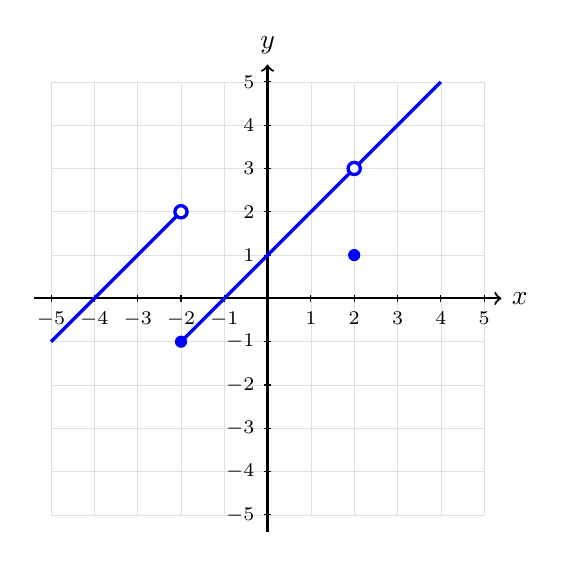
\begin{tikzpicture}[scale=0.55]
  \gridaxes{5}
  \draw[very thick,blue] (-5,-1)--(-2,2);
  \fill[white](-2,2) circle(4pt); \draw[very thick,blue](-2,2) circle(4pt);
  \draw[very thick,blue] (-2,-1)--(4,5);
  \fill[blue](-2,-1) circle(4pt);
  \fill[white](2,3) circle(4pt); \draw[very thick,blue](2,3) circle(4pt);
  \fill[blue](2,1) circle(4pt);
\end{tikzpicture}
\end{center}

\textbf{(a)} $\displaystyle\lim_{x \to -2^-} f(x) = \underline{\hspace{1.8cm}}$\quad
\textbf{(b)} $\displaystyle\lim_{x \to -2^+} f(x) = \underline{\hspace{1.8cm}}$\quad
\textbf{(c)} $\displaystyle\lim_{x \to -2} f(x) = \underline{\hspace{1.8cm}}$

\medskip
\textbf{(d)} $f(-2) = \underline{\hspace{1.8cm}}$\quad
\textbf{(e)} $\displaystyle\lim_{x \to 2} f(x) = \underline{\hspace{1.8cm}}$\quad
\textbf{(f)} $f(2) = \underline{\hspace{1.8cm}}$

\bigskip
\newpage
\textbf{2.}\quad Use the graph of $g$ below (the dashed line is a vertical asymptote).

\begin{center}
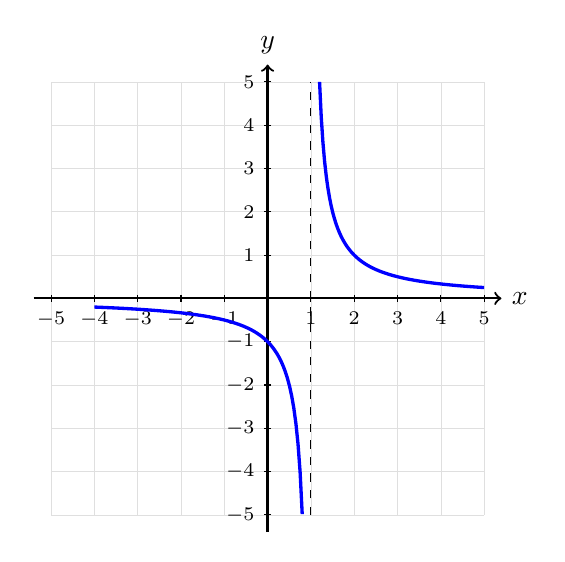
\begin{tikzpicture}[scale=0.55]
  \gridaxes{5}
  \draw[dashed] (1,-5)--(1,5);
  \draw[very thick,blue,domain=-4:0.8,samples=100] plot(\x,{1/(\x-1)});
  \draw[very thick,blue,domain=1.2:5,samples=100] plot(\x,{1/(\x-1)});
\end{tikzpicture}
\end{center}

\textbf{(a)} $\displaystyle\lim_{x \to 1^-} g(x) = \underline{\hspace{1.8cm}}$\quad
\textbf{(b)} $\displaystyle\lim_{x \to 1^+} g(x) = \underline{\hspace{1.8cm}}$\quad
\textbf{(c)} $\displaystyle\lim_{x \to 1} g(x) = \underline{\hspace{1.8cm}}$

\medskip
\textbf{(d)} Is $g(1)$ defined? \underline{\hspace{2.5cm}}\quad
\textbf{(e)} $\displaystyle\lim_{x \to +\infty} g(x) = \underline{\hspace{1.8cm}}$

\newpage
\textbf{3.}\quad Use the graph of $h$ below (the dashed lines are horizontal asymptotes).

\begin{center}
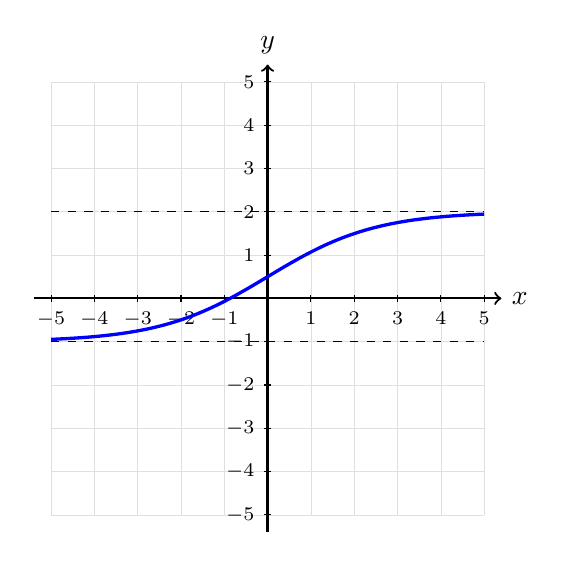
\begin{tikzpicture}[scale=0.55]
  \gridaxes{5}
  \draw[dashed] (-5,2)--(5,2);
  \draw[dashed] (-5,-1)--(5,-1);
  \draw[very thick,blue,domain=-5:5,samples=120] plot(\x,{2-3/(1+exp(0.8*\x))});
\end{tikzpicture}
\end{center}

\textbf{(a)} $\displaystyle\lim_{x \to +\infty} h(x) = \underline{\hspace{1.8cm}}$\quad
\textbf{(b)} $\displaystyle\lim_{x \to -\infty} h(x) = \underline{\hspace{1.8cm}}$

\medskip
\textbf{(c)} As $x \to +\infty$, does $h(x)$ ever actually \emph{equal} its limit, or only approach it? Explain.
\wl

\bigskip
\newpage
\textbf{4.}\quad \textbf{Putting it together.} Use the graph of $f$ below (the dashed line is a vertical
asymptote).

\begin{center}
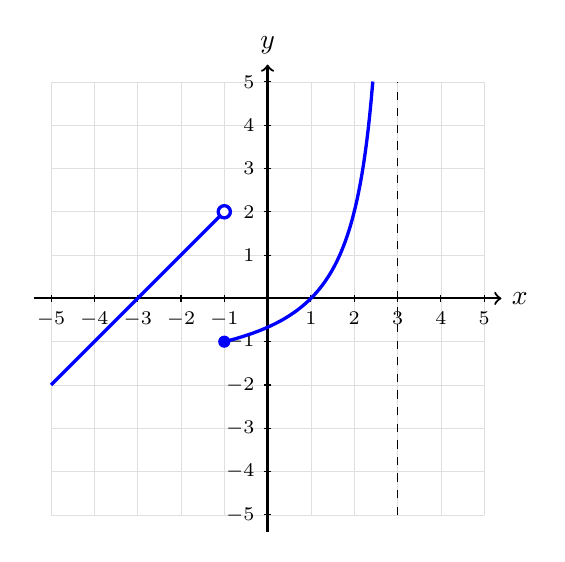
\begin{tikzpicture}[scale=0.55]
  \gridaxes{5}
  \draw[dashed] (3,-5)--(3,5);
  \draw[very thick,blue] (-5,-2)--(-1,2);
  \fill[white](-1,2) circle(4pt); \draw[very thick,blue](-1,2) circle(4pt);
  \fill[blue](-1,-1) circle(4pt);
  \draw[very thick,blue,domain=-1:2.43,samples=100] plot(\x,{4/(3-\x)-2});
\end{tikzpicture}
\end{center}

\textbf{(a)} $\displaystyle\lim_{x \to -1^-} f(x) = \underline{\hspace{1.6cm}}$\quad
\textbf{(b)} $\displaystyle\lim_{x \to -1^+} f(x) = \underline{\hspace{1.6cm}}$\quad
\textbf{(c)} $\displaystyle\lim_{x \to -1} f(x) = \underline{\hspace{1.6cm}}$

\medskip
\textbf{(d)} $f(-1) = \underline{\hspace{1.6cm}}$\quad
\textbf{(e)} $\displaystyle\lim_{x \to 3^-} f(x) = \underline{\hspace{1.6cm}}$

\medskip
\textbf{(f)} Does $\displaystyle\lim_{x \to 3} f(x)$ exist as a (finite) number? Explain.
\wl

% ===========================================================================
\newpage
\section*{Part 2 --- Explain in words}

\textbf{5.}\quad Can a limit \emph{exist} at a point where $f$ is \emph{undefined}? Explain, and give (or sketch)
an example.

\vspace{17em}

\textbf{6.}\quad Explain the difference between saying ``$\displaystyle\lim_{x \to a} f(x)$ does not exist'' and
saying ``$f(a)$ is undefined.'' Give an example of each.


% ===========================================================================
\newpage
\section*{Part 3 --- Sketch a graph to match}
With a \textbf{pencil}, draw \textbf{any} function whose graph satisfies all the given conditions. (There are infinitely many correct answers.)

\bigskip
\textbf{7.}\quad $\displaystyle\lim_{x \to 1^-} f(x) = 3$,\quad $\displaystyle\lim_{x \to 1^+} f(x) = -1$,\quad
$f(1) = 0$.

\begin{center}
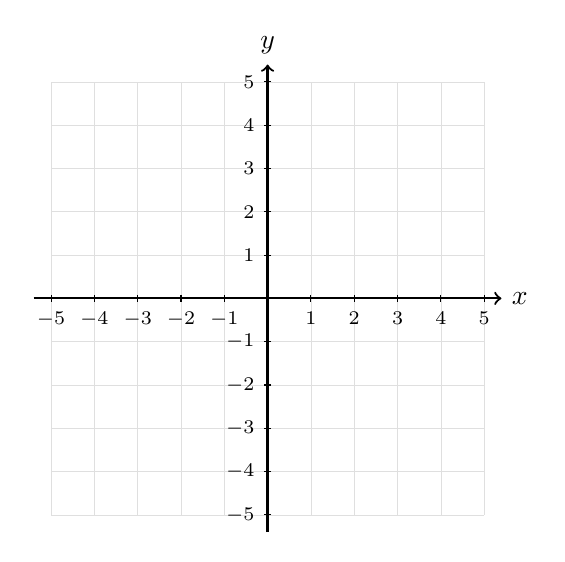
\begin{tikzpicture}[scale=0.55]\gridaxes{5}\end{tikzpicture}
\end{center}

\textbf{8.}\quad $\displaystyle\lim_{x \to 2} g(x) = 4$ \;(the two-sided limit exists),\quad but\quad $g(2) = 1$.

\begin{center}
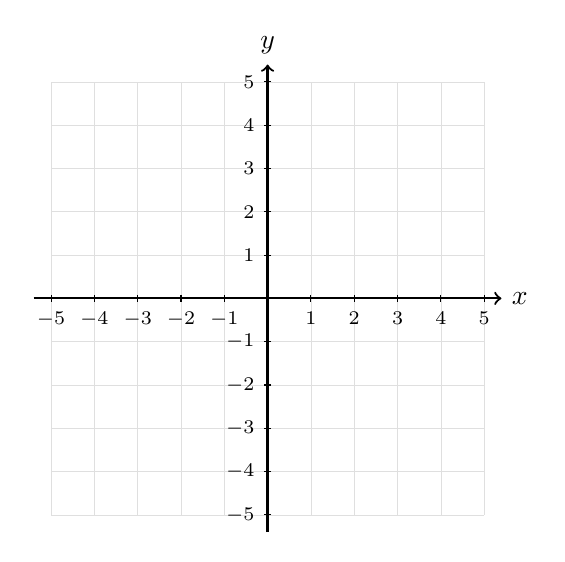
\begin{tikzpicture}[scale=0.55]\gridaxes{5}\end{tikzpicture}
\end{center}

\newpage
\textbf{9.}\quad $\displaystyle\lim_{x \to 0^-} h(x) = -\infty$,\quad $\displaystyle\lim_{x \to 0^+} h(x) =
+\infty$,\quad and\quad $\displaystyle\lim_{x \to +\infty} h(x) = 2$.

\begin{center}
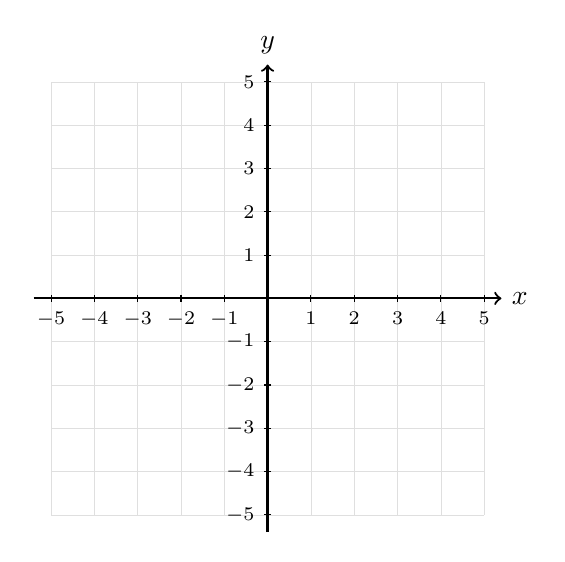
\begin{tikzpicture}[scale=0.55]\gridaxes{5}\end{tikzpicture}
\end{center}

% ===========================================================================
\newpage
\section*{Part 4 --- Find the limit with algebra}
\textit{First try substituting. If you get an ordinary number, that is the limit. If you get $\tfrac{0}{0}$,
factor and cancel first. For one-sided and infinite limits, think about the sign and size near the point.}

\medskip
\textbf{10.}\quad Find each limit. Show your steps.

\medskip
\textbf{(a)}\quad $\displaystyle\lim_{x \to 2} (x^2 + 3x - 1)$

\vspace{17em}

\textbf{(b)}\quad $\displaystyle\lim_{x \to -3} \frac{x^2 + x - 6}{x + 3}$
\vspace{17em}

\newpage
\textbf{(c)}\quad $\displaystyle\lim_{x \to 2} \frac{x^2 - x - 2}{x - 2}$
\vspace{17em}

\textbf{(d)}\quad For $\;f(x) = \begin{cases} x + 3 & \text{if } x < 1 \\ x^2 + 1 & \text{if } x \ge 1
\end{cases}$\;, find $\displaystyle\lim_{x \to 1^-} f(x)$, $\displaystyle\lim_{x \to 1^+} f(x)$, and
$\displaystyle\lim_{x \to 1} f(x)$.
\vspace{17em}

\newpage
\textbf{(e)}\quad $\displaystyle\lim_{x \to 3^+} \frac{1}{x - 3}$ \;and\; $\displaystyle\lim_{x \to 3^-}
\frac{1}{x - 3}$. \;Does $\displaystyle\lim_{x \to 3} \frac{1}{x-3}$ exist?
\vspace{17em}

\textbf{(f)}\quad $\displaystyle\lim_{x \to +\infty} \frac{3x^2 + 2x}{x^2 - 5}$
\vspace{17em}

\medskip
\newpage
\textbf{(g)}\quad $\bigstar$\quad $\displaystyle\lim_{x \to 0} \frac{\sqrt{x + 9} - 3}{x}$
\;\textit{(hint: multiply top and bottom by $\sqrt{x+9} + 3$).}
\vspace{17em}

% ===========================================================================
\newpage
\section*{Part 5 --- A real-world one-sided limit}
A parking garage charges by the hour, and you pay for the whole hour you are in:
\[
  C(t) = \begin{cases}
    \$4 & \text{if } 0 < t \le 1 \\
    \$7 & \text{if } 1 < t \le 2 \\
    \$10 & \text{if } 2 < t \le 3
  \end{cases}
\]
where $t$ is the number of hours parked. Its graph is a ``staircase'':

\begin{center}
\begin{tikzpicture}[scale=0.62]
  \draw[->] (0,0)--(4,0) node[right]{$t$ (hours)};
  \draw[->] (0,0)--(0,12) node[above]{cost (\$)};
  \foreach \t in {1,2,3}{\draw (\t,0.12)--(\t,-0.12) node[below]{\scriptsize$\t$};}
  \foreach \c in {4,7,10}{\draw (0.12,\c)--(-0.12,\c) node[left]{\scriptsize\$\c};}
  \draw[very thick,blue] (0,4)--(1,4); \fill[white](0,4)circle(3pt);\draw[blue,thick](0,4)circle(3pt); \fill[blue](1,4)circle(3pt);
  \draw[very thick,blue] (1,7)--(2,7); \fill[white](1,7)circle(3pt);\draw[blue,thick](1,7)circle(3pt); \fill[blue](2,7)circle(3pt);
  \draw[very thick,blue] (2,10)--(3,10); \fill[white](2,10)circle(3pt);\draw[blue,thick](2,10)circle(3pt); \fill[blue](3,10)circle(3pt);
\end{tikzpicture}
\end{center}

\textbf{11.}\quad
\textbf{(a)} $\displaystyle\lim_{t \to 2^-} C(t) = \underline{\hspace{1.8cm}}$\quad
\textbf{(b)} $\displaystyle\lim_{t \to 2^+} C(t) = \underline{\hspace{1.8cm}}$\quad
\textbf{(c)} $C(2) = \underline{\hspace{1.8cm}}$

\medskip
\textbf{(d)} Does $\displaystyle\lim_{t \to 2} C(t)$ exist? Explain what the two one-sided limits \emph{mean} for
someone parking right around $2$ hours.
\wls{3}

% ===========================================================================
\newpage
\section*{Notebook Artifact}

\bigskip
\textbf{N2.}\quad If you used the internet or AI, describe how you used it.
\wls{5}

\end{document}